%% Chapter 16: Observability and Observers
%% IEEE-format Control Systems Textbook
%% Self-contained chapter with complete derivations and practical experiments

\chapter{Observability and Observers}
\label{ch:observability}

\begin{quote}
\textit{``The observer problem is dual to the regulator problem; the two problems have exactly the same mathematical structure.''} --- Rudolf E. Kalman, 1960
\end{quote}

\section{Historical Motivation: The Hidden State Problem}

\subsection{The Fundamental Challenge of State Estimation}

The development of modern control theory in the late 1950s and early 1960s brought both unprecedented power and an unexpected challenge. State-space methods, championed by Rudolf Kalman and others, offered a systematic framework for designing controllers with optimal performance characteristics. State feedback, where the control input $u = -Kx$ is computed directly from the full state vector $x$, promised precise pole placement and optimal regulation. However, this elegant theory confronted a practical reality that threatened to undermine its applicability: \textit{in most real systems, we cannot measure all the states}.

Consider a DC motor driving a robotic arm. The state-space model requires knowledge of both position $\theta$ and angular velocity $\dot{\theta}$. While position can be measured directly with an encoder, measuring velocity precisely is far more challenging. Tachometers add cost, complexity, and mechanical coupling issues. Differentiating the position signal introduces noise that can destabilize the control system. The gap between the theoretical requirement for full-state feedback and the practical limitation of partial measurements seemed insurmountable.

\begin{historicalbox}[Kalman's Dual Discovery and Luenberger's Observer (1960--1964)]
In 1960, Rudolf Kalman published a landmark paper recognizing a beautiful duality in control mathematics: the question ``Can we drive the system anywhere?'' (controllability) is mathematically equivalent to ``Can we determine where the system has been?'' (observability). This duality meant that every theorem about controllability had a corresponding theorem about observability. Four years later, David G. Luenberger provided the practical implementation in his 1964 paper ``Observing the State of a Linear System,'' introducing the state observer that bears his name. Luenberger's key insight was elegant: if we know the system's model and have access to both input and output, we can build a ``copy'' of the system that converges to the true state by feeding back the difference between predicted and actual measurements.
\end{historicalbox}

\subsection{Kalman's Dual Discovery (1960)}

In 1960, Rudolf Kalman published a landmark paper that addressed this challenge from a fundamental mathematical perspective. While developing the theory of controllability---the question of whether control inputs could steer a system to any desired state---Kalman recognized a beautiful duality in the mathematics. The question ``Can we drive the system anywhere?'' was mathematically equivalent to asking ``Can we determine where the system has been?''

This second question is \textbf{observability}: given measurements of a system's outputs over some time interval, can we uniquely determine what the system's internal state was? Kalman showed that observability is the dual concept to controllability. \textbf{Controllability} asks whether the input $u(t)$ can steer the state $x$ to any desired value, while \textbf{observability} asks whether the output history $y(\tau)$ for $\tau \in [0, t]$ can reveal the initial state $x(0)$.

These two properties are linked by a profound mathematical duality. For a system described by $(A, B, C, D)$, the pair $(A, B)$ is controllable if and only if $(A^T, B^T)$ is observable, and the pair $(A, C)$ is observable if and only if $(A^T, C^T)$ is controllable.

This duality meant that every theorem about controllability had a corresponding theorem about observability, and every technique for controller design had a dual technique for observer design.

\subsection{Luenberger's Observer (1964)}

While Kalman established the theoretical foundations, it was David G. Luenberger who provided the practical solution. In his 1964 paper ``Observing the State of a Linear System,'' Luenberger introduced what is now called the \textbf{Luenberger observer} (or state observer).

Luenberger's key insight was elegant: if we know the system's model $(A, B, C)$ and we have access to both the input $u$ and output $y$, we can build a ``copy'' of the system in software or hardware. This copy, running in parallel with the real system, uses the same input $u$ and compares its predicted output with the actual measured output $y$. Any discrepancy indicates that the copy's internal state estimate differs from the true state. By feeding this error back into the copy with appropriate gain, the estimate can be made to converge to the true state.

The observer takes the form:
\begin{equation}
\dot{\hat{x}} = A\hat{x} + Bu + L(y - C\hat{x})
\label{eq:luenberger_observer_intro}
\end{equation}

where $\hat{x}$ is the estimated state and $L$ is the observer gain matrix. The term $(y - C\hat{x})$ represents the ``innovation''---the difference between what we measure and what we predicted. The gain $L$ determines how aggressively the observer corrects its estimate based on this innovation.

\subsection{Aerospace Applications: Apollo Navigation}

The Apollo program provided one of the most dramatic demonstrations of state estimation in action. The challenge of navigating a spacecraft to the Moon and back required continuous knowledge of position and velocity in three-dimensional space---six state variables in all. However, the spacecraft's sensors provided only limited measurements: angles to known stars, range and range-rate to Earth-based tracking stations, and occasionally, angles to landmarks on the lunar surface.

The Apollo guidance computer implemented a sophisticated state estimator (specifically, a Kalman filter, which we will study in Chapter 18) that fused these partial measurements to produce a complete estimate of the spacecraft's state. This estimated state was then used for all navigation and control decisions. The success of Apollo demonstrated that state estimation was not merely a theoretical curiosity but an essential enabling technology for advanced control systems.

Consider the estimation problem during lunar orbit insertion: the spacecraft's position and velocity had to be known precisely to execute the burn that would capture the spacecraft into lunar orbit. Direct measurement of all six states was impossible, but by processing sequences of angular measurements to known stars and landmarks, combined with knowledge of the spacecraft's dynamics (gravitational attraction of the Moon and Earth), the navigation filter could reconstruct the full state with remarkable accuracy.

\subsection{Submarine Target Motion Analysis}

Another compelling application of observability theory emerged from naval warfare: target motion analysis (TMA) for submarines. A submarine tracking a surface target faces a challenging estimation problem. The submarine's passive sonar can measure the bearing to the target (the direction from which sound arrives) but cannot directly measure range or target velocity without going active and revealing its position.

The target motion analysis problem asks: given a sequence of bearing measurements over time, can we determine the target's position, course, and speed? This is precisely a question of observability. The answer depends on the geometry and the submarine's maneuvers. If the submarine maintains a steady course, the system is often unobservable---many different target trajectories are consistent with the observed bearing measurements. However, if the submarine maneuvers (changes course), the resulting bearing changes provide additional information that can make the system observable.

This application illustrates a key insight: observability is not just a property of the system being observed, but also depends on how we interact with it. The submarine's own maneuvers affect the observability of the target's state. This concept extends broadly: in many systems, careful choice of inputs or operating conditions can improve observability.

\subsection{The Key Insight}

The fundamental insight from this historical development is both simple and profound:

\begin{quote}
\textit{If a system is observable, its complete internal state can be reconstructed from a history of output measurements, even if we can never measure those internal states directly.}
\end{quote}

This means that the requirement for state feedback does not actually require direct measurement of all states. Instead, we need only a system that is observable (a property we can check mathematically), an observer that uses available measurements to estimate unmeasured states, and sufficient time for the observer's estimates to converge to the true states.

The development of observability theory and state observers transformed state-space control from an elegant but impractical theory into a practical engineering discipline that underlies much of modern control system design.

%% ============================================================================
\section{Modern Applications}
%% ============================================================================

The principles of observability and state estimation, developed in the 1960s for aerospace applications, have become ubiquitous in modern engineering. Today, observers are embedded in billions of devices, from smartphones to electric vehicles. This section surveys several contemporary applications.

\subsection{GPS Receivers}

Global Positioning System (GPS) receivers present a fascinating estimation problem. The receiver measures the time-of-arrival of signals from multiple satellites, from which it computes ``pseudoranges''---approximate distances to each satellite. However, these pseudoranges are corrupted by several error sources: atmospheric delays, multipath reflections, and most significantly, clock bias between the receiver's local oscillator and the satellite atomic clocks.

A GPS receiver implements a state estimator that tracks not only the receiver's position (three states: $x$, $y$, $z$) and velocity (three states: $\dot{x}$, $\dot{y}$, $\dot{z}$) but also the clock bias and its drift rate (two additional states). By processing pseudorange and Doppler measurements from multiple satellites, the receiver estimates all eight states, providing accurate position and velocity even though none of these states is directly measured.

\subsection{Motor Control: Velocity Estimation from Position}

Electric motor drives routinely estimate velocity from position encoder measurements. While encoders provide precise position information, directly differentiating the encoder signal to obtain velocity produces a noisy, quantized signal that is unsuitable for high-performance velocity control.

Instead, modern motor drives implement velocity observers that combine the encoder position with knowledge of the motor's electrical and mechanical dynamics. The observer produces a smooth velocity estimate that enables tight servo performance. This approach is particularly important in industrial robots requiring precise velocity control for smooth motion, disk drive head positioning requiring vibration-free settling, and electric vehicle traction motors requiring smooth torque delivery.

We will implement exactly such an observer in the practical experiment section of this chapter.

\subsection{Battery State-of-Charge Estimation}

Electric vehicles and portable electronics rely on accurate estimation of battery state-of-charge (SoC)---the percentage of remaining capacity. Direct measurement of SoC is essentially impossible; one cannot simply ``look inside'' an electrochemical cell to determine its charge level.

However, battery voltage, current, and temperature can be measured. An observer that incorporates an electrochemical model of the battery can estimate SoC from these measurements. The challenge is significant: battery dynamics are nonlinear, temperature-dependent, and subject to aging effects. Modern battery management systems implement extended Kalman filters or other nonlinear observers to track not only SoC but also state-of-health parameters that change over the battery's lifetime.

\subsection{Soft Sensors in Chemical Processes}

In chemical process industries, many important quantities cannot be measured directly or can only be measured with long time delays. Product composition, for example, might be determined only by laboratory analysis of samples, with results available hours after the sample was taken. Biomass concentration in fermentation processes may be measurable only through offline assays.

``Soft sensors'' use observers based on process models and real-time measurements of readily available quantities (temperature, pressure, flow rates) to estimate these hard-to-measure variables. These estimates enable real-time control that would otherwise be impossible.

%% ============================================================================
\section{Mathematical Foundation}
%% ============================================================================

Having motivated the problem historically and illustrated its modern relevance, we now develop the mathematical theory of observability and observer design. The treatment parallels the development of controllability in Chapter 15, exploiting the duality between the two concepts.

\subsection{System Description}

We consider a linear time-invariant (LTI) continuous-time system in state-space form:
\begin{align}
\dot{x}(t) &= Ax(t) + Bu(t) \label{eq:state_equation}\\
y(t) &= Cx(t) + Du(t) \label{eq:output_equation}
\end{align}

The variables and matrices are defined in Table~\ref{tab:state_space_variables}.

\begin{table}[ht]
\centering
\caption{State-Space System Variables and Matrices}
\label{tab:state_space_variables}
\begin{tabular}{@{}cl@{}}
\toprule
\textbf{Symbol} & \textbf{Description} \\
\midrule
$x(t) \in \mathbb{R}^n$ & State vector \\
$u(t) \in \mathbb{R}^m$ & Input vector \\
$y(t) \in \mathbb{R}^p$ & Output vector \\
$A \in \mathbb{R}^{n \times n}$ & System matrix \\
$B \in \mathbb{R}^{n \times m}$ & Input matrix \\
$C \in \mathbb{R}^{p \times n}$ & Output matrix \\
$D \in \mathbb{R}^{p \times m}$ & Feedthrough matrix \\
\bottomrule
\end{tabular}
\end{table}

For the study of observability, we focus on the pair $(A, C)$. The input $u(t)$ is assumed known, and for simplicity in developing the theory, we often set $u(t) = 0$ and $D = 0$.

\subsection{Definition of Observability}

\begin{definition}[Observability]
The system (\ref{eq:state_equation})--(\ref{eq:output_equation}), or equivalently the pair $(A, C)$, is said to be \textbf{observable} if for any unknown initial state $x(0) = x_0$, there exists a finite time $t_1 > 0$ such that knowledge of the input $u(t)$ and output $y(t)$ over the interval $[0, t_1]$ suffices to uniquely determine $x_0$.
\end{definition}

An equivalent formulation focuses on distinguishability: a system is observable if and only if no two distinct initial states produce identical output trajectories under the same input sequence.

\begin{definition}[Unobservable State]
A state $x_0 \neq 0$ is \textbf{unobservable} if the system initialized at $x_0$ with $u(t) = 0$ produces $y(t) = 0$ for all $t \geq 0$. The system is observable if and only if the only unobservable state is $x_0 = 0$.
\end{definition}

\subsection{The Observability Matrix}

The key to testing observability is the \textbf{observability matrix}, constructed from $A$ and $C$:

\begin{definition}[Observability Matrix]
The observability matrix for the pair $(A, C)$ is defined as:
\begin{equation}
\mathcal{O} = \begin{bmatrix}
C \\
CA \\
CA^2 \\
\vdots \\
CA^{n-1}
\end{bmatrix} \in \mathbb{R}^{np \times n}
\label{eq:observability_matrix}
\end{equation}
\end{definition}

This matrix stacks the output at time zero ($y(0) = Cx_0$), the first derivative of the output ($\dot{y}(0) = CAx_0$), and so forth, up to the $(n-1)$-th derivative.

\begin{theorem}[Observability Rank Condition]
The pair $(A, C)$ is observable if and only if the observability matrix $\mathcal{O}$ has full column rank:
\begin{equation}
\text{rank}(\mathcal{O}) = n
\label{eq:observability_rank}
\end{equation}
\end{theorem}

\begin{proof}
Consider the autonomous system ($u = 0$) with initial condition $x(0) = x_0$. The output and its derivatives at $t = 0$ are:
\begin{align}
y(0) &= Cx_0 \\
\dot{y}(0) &= C\dot{x}(0) = CAx_0 \\
\ddot{y}(0) &= CA\dot{x}(0) = CA^2x_0 \\
&\vdots \\
y^{(n-1)}(0) &= CA^{n-1}x_0
\end{align}

This can be written in matrix form as:
\begin{equation}
\begin{bmatrix}
y(0) \\
\dot{y}(0) \\
\vdots \\
y^{(n-1)}(0)
\end{bmatrix}
= \mathcal{O} x_0
\end{equation}

If $\text{rank}(\mathcal{O}) = n$, then $\mathcal{O}$ has a left inverse $\mathcal{O}^\dagger = (\mathcal{O}^T\mathcal{O})^{-1}\mathcal{O}^T$, and we can solve for $x_0$:
\begin{equation}
x_0 = \mathcal{O}^\dagger \begin{bmatrix}
y(0) \\
\dot{y}(0) \\
\vdots \\
y^{(n-1)}(0)
\end{bmatrix}
\end{equation}

Thus, the initial state can be uniquely determined from the output and its first $n-1$ derivatives, proving observability.

Conversely, if $\text{rank}(\mathcal{O}) < n$, then $\mathcal{O}$ has a non-trivial null space. Any $x_0 \neq 0$ in the null space of $\mathcal{O}$ satisfies $\mathcal{O}x_0 = 0$, meaning $Cx_0 = CAx_0 = \cdots = CA^{n-1}x_0 = 0$. By the Cayley-Hamilton theorem, $CA^k x_0 = 0$ for all $k \geq 0$, and hence $y(t) = Ce^{At}x_0 = 0$ for all $t$. Such an $x_0$ is unobservable, proving the system is not observable.
\end{proof}

\subsection{Duality Between Controllability and Observability}

The controllability and observability concepts are related by a beautiful mathematical duality.

\begin{theorem}[Duality Theorem]
The pair $(A, C)$ is observable if and only if the pair $(A^T, C^T)$ is controllable.
\end{theorem}

\begin{proof}
The controllability matrix for the pair $(A^T, C^T)$ is:
\begin{equation}
\mathcal{C}_{A^T, C^T} = \begin{bmatrix}
C^T & A^TC^T & (A^T)^2C^T & \cdots & (A^T)^{n-1}C^T
\end{bmatrix}
\end{equation}

Taking the transpose:
\begin{equation}
\mathcal{C}_{A^T, C^T}^T = \begin{bmatrix}
C \\ CA \\ CA^2 \\ \vdots \\ CA^{n-1}
\end{bmatrix} = \mathcal{O}_{A,C}
\end{equation}

Since a matrix and its transpose have the same rank, $\text{rank}(\mathcal{C}_{A^T, C^T}) = \text{rank}(\mathcal{O}_{A,C})$. The controllability rank condition for $(A^T, C^T)$ is equivalent to the observability rank condition for $(A, C)$.
\end{proof}

This duality has profound practical implications. Any result for controllability immediately yields a corresponding result for observability by transposition. Any algorithm for computing controller gains can be adapted for observer gains. The theoretical development is essentially ``two for the price of one.''

\begin{table}[ht]
\centering
\caption{Duality Between Controllability and Observability}
\label{tab:duality}
\begin{tabular}{@{}ll@{}}
\toprule
\textbf{Controllability} & \textbf{Observability} \\
\midrule
Pair $(A, B)$ & Pair $(A, C)$ \\
Can input reach all states? & Can output reveal all states? \\
Controllability matrix $\mathcal{C} = [B\; AB\; \cdots\; A^{n-1}B]$ & Observability matrix $\mathcal{O} = [C;\; CA;\; \cdots;\; CA^{n-1}]^T$ \\
$\text{rank}(\mathcal{C}) = n$ & $\text{rank}(\mathcal{O}) = n$ \\
State feedback: $u = -Kx$ & Observer: $\dot{\hat{x}} = A\hat{x} + Bu + L(y-C\hat{x})$ \\
Closed-loop: $A - BK$ & Error dynamics: $A - LC$ \\
Place eigenvalues of $A-BK$ & Place eigenvalues of $A-LC$ \\
\bottomrule
\end{tabular}
\end{table}

\subsection{The Luenberger Observer}

We now develop the Luenberger observer, which uses output measurements to estimate the unmeasured states of an observable system.

\subsubsection{Observer Structure}

The observer is a dynamical system that runs alongside (or in software, simulating) the plant. It receives the same input $u(t)$ as the plant and uses the output measurement $y(t)$ to correct its state estimate:

\begin{equation}
\dot{\hat{x}} = A\hat{x} + Bu + L(y - C\hat{x})
\label{eq:luenberger_observer}
\end{equation}

In this equation, $\hat{x}(t) \in \mathbb{R}^n$ is the estimated state, $L \in \mathbb{R}^{n \times p}$ is the observer gain matrix, and the term $y - C\hat{x}$ is the \textbf{output estimation error} (or ``innovation'').

The observer can be rewritten as:
\begin{equation}
\dot{\hat{x}} = (A - LC)\hat{x} + Bu + Ly
\label{eq:observer_standard_form}
\end{equation}

This shows that the observer is itself an LTI system with system matrix $(A-LC)$, driven by inputs $u$ and $y$.

\subsubsection{Error Dynamics}

The key to understanding observer performance is the \textbf{state estimation error}:
\begin{equation}
e(t) = x(t) - \hat{x}(t)
\end{equation}

Taking the derivative:
\begin{align}
\dot{e} &= \dot{x} - \dot{\hat{x}} \\
&= (Ax + Bu) - (A\hat{x} + Bu + L(y - C\hat{x})) \\
&= A(x - \hat{x}) - L(Cx - C\hat{x}) \\
&= Ae - LCe \\
&= (A - LC)e
\label{eq:error_dynamics}
\end{align}

This is a remarkable result: the error dynamics are governed by the autonomous system with matrix $(A - LC)$, and they are \textit{independent of the actual system trajectory and input}. The error evolves according to:
\begin{equation}
e(t) = e^{(A-LC)t} e(0)
\end{equation}

\subsubsection{Observer Pole Placement}

If the eigenvalues of $(A - LC)$ all have negative real parts, then $e(t) \to 0$ as $t \to \infty$, regardless of the initial error $e(0) = x(0) - \hat{x}(0)$. The rate of convergence depends on the eigenvalue locations: more negative eigenvalues yield faster convergence.

\begin{theorem}[Observer Pole Placement]
If the pair $(A, C)$ is observable, then the observer gain $L$ can be chosen to place the eigenvalues of $(A - LC)$ at any desired locations in the complex plane.
\end{theorem}

\begin{proof}
By duality, the pair $(A, C)$ is observable if and only if $(A^T, C^T)$ is controllable. We know from Chapter 15 that if $(A^T, C^T)$ is controllable, we can find a matrix $K_d$ such that the eigenvalues of $A^T - C^T K_d$ are at any desired locations.

Note that:
\begin{equation}
A^T - C^T K_d = (A - K_d^T C)^T
\end{equation}

Since a matrix and its transpose have identical eigenvalues, setting $L = K_d^T$ places the eigenvalues of $A - LC$ at the same desired locations.
\end{proof}

\textbf{Practical Considerations for Observer Pole Placement:}

Several practical considerations guide the selection of observer pole locations. First, observer poles should be placed faster than the controller poles, typically 2--10 times faster, ensuring that the state estimates converge before they significantly affect control performance. However, extremely fast observer poles amplify measurement noise, creating a fundamental trade-off between convergence speed and noise sensitivity. Finally, if the plant has stable but slow modes, the observer must be faster than those modes to estimate the corresponding states before they contribute significantly to the response.

\subsection{Observer Design by Pole Placement}

For a single-output system ($p = 1$), the observer pole placement problem can be solved using methods analogous to controller design. One approach uses the duality and Ackermann's formula.

\textbf{Dual Ackermann's Formula:} For a single-output system, the observer gain is given by:
\begin{equation}
L = \alpha_o(A) \mathcal{O}^{-1} \begin{bmatrix} 0 \\ 0 \\ \vdots \\ 0 \\ 1 \end{bmatrix}
\label{eq:ackermann_observer}
\end{equation}

where $\alpha_o(s) = (s - \lambda_1)(s - \lambda_2) \cdots (s - \lambda_n)$ is the desired observer characteristic polynomial and $\mathcal{O}$ is the observability matrix.

\begin{algorithm}
\caption{Observer Pole Placement}
\begin{algorithmic}[1]
\Require System matrices $A$, $C$; desired observer poles $\lambda_1, \lambda_2, \ldots, \lambda_n$
\Ensure Observer gain matrix $L$
\State Define system matrix $A$ and output matrix $C$
\State Specify desired observer pole locations (faster than controller poles)
\State Compute observer gain: $L \leftarrow \textsc{Place}(A^T, C^T, \text{poles})^T$
\State Verify eigenvalues of $(A - LC)$ match desired poles
\State \Return $L$
\end{algorithmic}
\end{algorithm}

\subsection{The Separation Principle}

A crucial question arises when combining state-feedback control with state estimation: does using estimated states instead of true states affect stability or performance guarantees? The separation principle provides a reassuring answer.

\begin{theorem}[Separation Principle]
Consider a state-feedback controller $u = -Kx$ designed assuming access to the true state $x$. When implemented using the estimated state from an asymptotically stable observer, $u = -K\hat{x}$, the closed-loop system remains stable if and only if both the state feedback $(A - BK)$ and the observer $(A - LC)$ are stable. Furthermore, the closed-loop eigenvalues are the union of the controller eigenvalues and the observer eigenvalues.
\end{theorem}

\begin{proof}
With observer-based control, the closed-loop dynamics are:
\begin{align}
\dot{x} &= Ax + Bu = Ax - BK\hat{x} = Ax - BK(x - e) = (A-BK)x + BKe \\
\dot{e} &= (A-LC)e
\end{align}

In matrix form:
\begin{equation}
\begin{bmatrix} \dot{x} \\ \dot{e} \end{bmatrix} = \underbrace{\begin{bmatrix} A-BK & BK \\ 0 & A-LC \end{bmatrix}}_{A_{cl}} \begin{bmatrix} x \\ e \end{bmatrix}
\label{eq:separation_principle}
\end{equation}

The closed-loop matrix $A_{cl}$ is block upper triangular. The eigenvalues of a block triangular matrix are the eigenvalues of its diagonal blocks. Therefore:
\begin{equation}
\text{eigenvalues}(A_{cl}) = \text{eigenvalues}(A-BK) \cup \text{eigenvalues}(A-LC)
\end{equation}

The system is stable if and only if all eigenvalues have negative real parts, which requires both $(A-BK)$ and $(A-LC)$ to be stable.
\end{proof}

The separation principle is remarkable: the controller design and observer design can be carried out \textit{independently}. The controller is designed assuming perfect state information, then the observer is designed to provide state estimates, and the combination is guaranteed to work.

\subsection{Observer-Based Control Implementation}

The complete observer-based control system has the following structure:

\textbf{Plant:}
\begin{align}
\dot{x} &= Ax + Bu \\
y &= Cx
\end{align}

\textbf{Observer:}
\begin{equation}
\dot{\hat{x}} = A\hat{x} + Bu + L(y - C\hat{x})
\end{equation}

\textbf{Control Law:}
\begin{equation}
u = -K\hat{x}
\end{equation}

Note that the observer requires knowledge of the input $u$, which depends on the estimated state $\hat{x}$. The complete observer-based controller, also known as a \textbf{compensator}, can be written as a dynamical system from measurement $y$ to control $u$:

\begin{align}
\dot{\hat{x}} &= (A - BK - LC)\hat{x} + Ly \\
u &= -K\hat{x}
\end{align}

This is a state-space realization of the compensator transfer function from $y$ to $u$.

\subsection{Transfer Function Interpretation}

The observer-based controller can be expressed as a transfer function:
\begin{equation}
K_{controller}(s) = K(sI - A + BK + LC)^{-1}L
\end{equation}

This connects state-space observer-based control to classical frequency-domain compensation. The observer-based controller implements a dynamic compensator whose order equals the plant order.

%% ============================================================================
\section{Practical Experiment: Motor Velocity Observer}
%% ============================================================================

\subsection{Objective}

In this experiment, we implement a Luenberger observer to estimate the angular velocity of a DC motor from position encoder measurements alone. We compare the observer-based velocity estimate against numerical differentiation, demonstrating the superior noise rejection of the observer approach.

\subsection{Required Equipment}

The experiment requires the following equipment: a DC motor with quadrature encoder (such as a Pololu 37D gearmotor with 64 CPR encoder), a motor driver (L298N or similar H-bridge), an Arduino Mega or similar microcontroller, a power supply appropriate for the motor, an oscilloscope or data logging capability, and a computer with Arduino IDE and MATLAB/Python for analysis.

\subsection{Motor Model}

A DC motor can be modeled with two states: angular position $\theta$ and angular velocity $\omega = \dot{\theta}$. For a motor with negligible electrical dynamics (small electrical time constant compared to mechanical), the mechanical dynamics are:

\begin{equation}
J\dot{\omega} + b\omega = K_t i = K_t \frac{V - K_e\omega}{R}
\end{equation}

where $J$ is the moment of inertia, $b$ is the viscous friction, $K_t$ is the torque constant, $K_e$ is the back-EMF constant, and $R$ is the armature resistance.

This simplifies to the first-order mechanical model:
\begin{equation}
\dot{\omega} = -\frac{b_{eff}}{J}\omega + \frac{K}{J}V
\end{equation}

where $b_{eff} = b + K_t K_e/R$ is the effective damping and $K = K_t/R$.

The state-space model with position and velocity as states is:
\begin{equation}
\begin{bmatrix} \dot{\theta} \\ \dot{\omega} \end{bmatrix}
= \begin{bmatrix} 0 & 1 \\ 0 & -b_{eff}/J \end{bmatrix}
\begin{bmatrix} \theta \\ \omega \end{bmatrix}
+ \begin{bmatrix} 0 \\ K/J \end{bmatrix} V
\end{equation}

With position measurement only:
\begin{equation}
y = \theta = \begin{bmatrix} 1 & 0 \end{bmatrix} \begin{bmatrix} \theta \\ \omega \end{bmatrix}
\end{equation}

\subsection{Observability Analysis}

For the motor model with $A = \begin{bmatrix} 0 & 1 \\ 0 & -a \end{bmatrix}$ (where $a = b_{eff}/J$) and $C = \begin{bmatrix} 1 & 0 \end{bmatrix}$:

\begin{equation}
\mathcal{O} = \begin{bmatrix} C \\ CA \end{bmatrix}
= \begin{bmatrix} 1 & 0 \\ 0 & 1 \end{bmatrix}
\end{equation}

The observability matrix is the identity matrix, which has rank 2. The system is observable! This means we can estimate velocity from position measurements.

\subsection{Observer Design}

Let the motor parameters be identified as $a = 10$ rad/s and $b = K/J = 50$ rad/s$^2$/V. We design an observer with poles at $s = -50$ and $s = -60$, making the observer 5--6 times faster than the motor's dominant time constant.

The observer gains are computed:
\begin{equation}
L = \begin{bmatrix} l_1 \\ l_2 \end{bmatrix}
\end{equation}

The observer characteristic polynomial is:
\begin{equation}
\det(sI - A + LC) = s^2 + (a + l_1)s + (l_2 + al_1) = (s+50)(s+60) = s^2 + 110s + 3000
\end{equation}

Matching coefficients:
\begin{align}
a + l_1 &= 110 \implies l_1 = 110 - 10 = 100 \\
l_2 + al_1 &= 3000 \implies l_2 = 3000 - 10 \times 100 = 2000
\end{align}

So $L = \begin{bmatrix} 100 \\ 2000 \end{bmatrix}$.

\subsection{Microcontroller Implementation}

The following algorithms describe the implementation of the velocity observer on a microcontroller. The implementation consists of three main components: initialization, encoder reading, and the observer update routine.

\begin{algorithm}
\caption{Motor Velocity Observer -- Initialization}
\begin{algorithmic}[1]
\Require System parameters $a$, $b$; observer gains $L_1$, $L_2$; sample time $T_s$
\State Initialize serial communication for data logging
\State Configure encoder pins as inputs with pull-up resistors
\State Configure motor PWM and direction pins as outputs
\State Attach interrupt handlers to encoder channels A and B
\State Configure timer for fixed sample rate (e.g., 1 kHz)
\State Initialize state estimates: $\hat{\theta} \leftarrow 0$, $\hat{\omega} \leftarrow 0$
\State Initialize comparison variables: $\theta_{prev} \leftarrow 0$, $\omega_{deriv} \leftarrow 0$
\end{algorithmic}
\end{algorithm}

\begin{algorithm}
\caption{Quadrature Encoder Interrupt Service Routine}
\begin{algorithmic}[1]
\Require Current encoder channel states A, B
\State Read current state: $s \leftarrow (A \ll 1) \lor B$
\State Look up increment from state transition table using previous and current states
\State Update encoder count: $\text{count} \leftarrow \text{count} + \text{increment}$
\State Store current state for next interrupt
\end{algorithmic}
\end{algorithm}

\begin{algorithm}
\caption{Luenberger Observer Update (Timer ISR)}
\begin{algorithmic}[1]
\Require Encoder count, system parameters $a$, $b$, observer gains $L_1$, $L_2$, sample time $T_s$
\State \textbf{// Read position measurement}
\State $\theta_{meas} \leftarrow \text{count} / \text{countsPerRad}$
\State
\State \textbf{// Numerical derivative with low-pass filter (for comparison)}
\State $\omega_{raw} \leftarrow (\theta_{meas} - \theta_{prev}) / T_s$
\State $\omega_{deriv} \leftarrow \alpha \cdot \omega_{raw} + (1 - \alpha) \cdot \omega_{deriv}$ \Comment{$\alpha \approx 0.2$}
\State $\theta_{prev} \leftarrow \theta_{meas}$
\State
\State \textbf{// Luenberger Observer}
\State \textbf{Prediction step:}
\State $\dot{\hat{\theta}} \leftarrow \hat{\omega}$
\State $\dot{\hat{\omega}} \leftarrow -a \cdot \hat{\omega} + b \cdot V$
\State
\State \textbf{Correction step:}
\State $\text{innovation} \leftarrow \theta_{meas} - \hat{\theta}$
\State $\dot{\hat{\theta}} \leftarrow \dot{\hat{\theta}} + L_1 \cdot \text{innovation}$
\State $\dot{\hat{\omega}} \leftarrow \dot{\hat{\omega}} + L_2 \cdot \text{innovation}$
\State
\State \textbf{Integration (Euler method):}
\State $\hat{\theta} \leftarrow \hat{\theta} + \dot{\hat{\theta}} \cdot T_s$
\State $\hat{\omega} \leftarrow \hat{\omega} + \dot{\hat{\omega}} \cdot T_s$
\State
\State \textbf{// Apply control signal to motor}
\State Set motor direction based on sign of $V$
\State Set motor PWM proportional to $|V|$
\end{algorithmic}
\end{algorithm}

\subsection{Experimental Procedure}

The experimental procedure consists of five phases. Begin with \textbf{system identification} by applying step inputs and measuring the motor's response to identify parameters $a$ and $b$. Next, proceed with \textbf{observer implementation} by uploading the observer code and running step response experiments. During \textbf{data collection}, log the estimated velocity $\hat{\omega}$, the numerical derivative $\omega_{deriv}$, and the applied voltage. For \textbf{comparison}, plot both velocity estimates; the observer estimate should be significantly smoother than the numerical derivative. Finally, conduct an \textbf{initial condition test} by initializing the observer with a large error (e.g., $\hat{\theta}(0) = 0$, $\hat{\omega}(0) = 100$) and observing convergence to the true state.

\subsection{Expected Results}

\begin{figure}[ht]
\centering
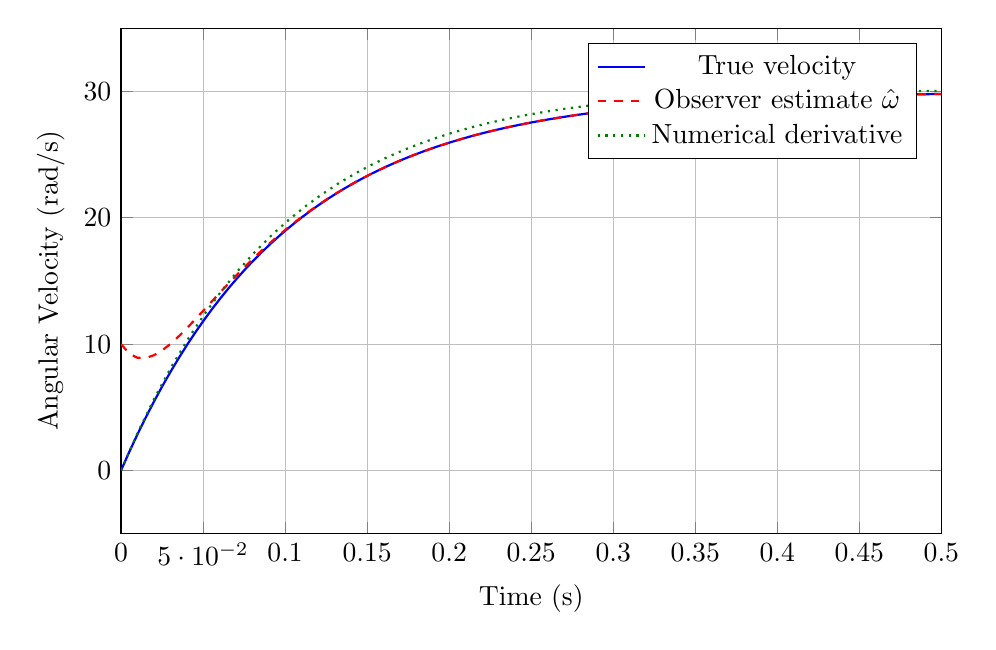
\begin{tikzpicture}
\begin{axis}[
    width=12cm,
    height=8cm,
    xlabel={Time (s)},
    ylabel={Angular Velocity (rad/s)},
    legend pos=north east,
    grid=both,
    xmin=0, xmax=0.5,
    ymin=-5, ymax=35
]

% True velocity (simulated)
\addplot[blue, thick, domain=0:0.5, samples=100]
    {30*(1 - exp(-10*x))};
\addlegendentry{True velocity}

% Observer estimate (converging)
\addplot[red, thick, dashed, domain=0:0.5, samples=100]
    {30*(1 - exp(-10*x)) + 10*exp(-50*x)};
\addlegendentry{Observer estimate $\hat{\omega}$}

% Numerical derivative (noisy - simulated with randomness would need data)
\addplot[green!50!black, thick, dotted, domain=0:0.5, samples=50]
    {30*(1 - exp(-10*x)) + 3*sin(200*x)*exp(-5*x)};
\addlegendentry{Numerical derivative}

\end{axis}
\end{tikzpicture}
\caption{Comparison of velocity estimation methods. The observer estimate (dashed red) tracks the true velocity (solid blue) smoothly, while numerical differentiation (dotted green) is corrupted by noise.}
\label{fig:observer_comparison}
\end{figure}

Several key observations emerge from this comparison. The observer estimate converges to the true velocity within approximately $5/(50) = 0.1$ seconds (five time constants of the observer). The numerical derivative is noisy, especially during rapid changes. In contrast, the observer provides smooth estimates suitable for feedback control.

%% ============================================================================
\section{Block Diagrams}
%% ============================================================================

\subsection{Basic Observer Structure}

\begin{figure}[ht]
\centering
\begin{tikzpicture}[auto, node distance=2cm, >=latex',
    block/.append style={sharp corners}]
    % Plant
    \node [block, minimum width=2.5cm, minimum height=1.5cm] (plant) {Plant\\$\dot{x} = Ax + Bu$\\$y = Cx$};

    % Observer
    \node [block, minimum width=3cm, minimum height=2cm, below=2cm of plant, fill=blue!10] (observer) {Observer\\$\dot{\hat{x}} = A\hat{x} + Bu$\\$+ L(y - C\hat{x})$};

    % Sum for innovation
    \node [sum, right=2cm of observer] (sum) {};

    % Input
    \node [input, left=2cm of plant] (input) {};
    \node [above=0.3cm of input] {$u$};

    % Output
    \node [output, right=2cm of plant] (output) {};
    \node [above=0.3cm of output] {$y$};

    % Connections
    \draw [->] (input) -- (plant) node[pos=0.5, above] {};
    \draw [->] (plant) -- (output);
    \draw [->] (input) |- ($(plant.west)!0.5!(observer.west) - (1cm,0)$) |- (observer.west);

    % Output to innovation sum
    \draw [->] (output) |- ($(sum) + (0,1.5cm)$) -- (sum) node[pos=0.9, right] {$+$};

    % Observer output to sum
    \node [block, right=0.5cm of observer, minimum width=1cm] (Cblock) {$C$};
    \draw [->] (observer) -- (Cblock);
    \draw [->] (Cblock) -| (sum) node[pos=0.9, above] {$-$};

    % Innovation back to observer
    \node [block, below=0.5cm of sum, minimum width=1cm] (Lblock) {$L$};
    \draw [->] (sum) -- (Lblock);
    \draw [->] (Lblock) -| ($(observer.south) + (1cm,0)$) -- ($(observer.east) - (0,0.5cm)$);

    % State estimate output
    \node [output, below=0.5cm of observer] (xhat_out) {};
    \draw [->] (observer.south) -- (xhat_out) node[below] {$\hat{x}$};

    % Labels
    \node [above=0.1cm of sum] {Innovation};

\end{tikzpicture}
\caption{Luenberger observer structure. The observer is a copy of the plant that uses the innovation signal $(y - C\hat{x})$ to correct its state estimate.}
\label{fig:observer_block}
\end{figure}

\subsection{Observer-Based Control System}

\begin{figure}[ht]
\centering
\begin{tikzpicture}[auto, node distance=2cm, >=latex',
    block/.append style={sharp corners}]
    % Reference
    \node [input] (ref) {};
    \node [above=0.2cm of ref] {$r$};

    % Sum for reference error (optional, for tracking)
    \node [sum, right=1cm of ref] (refsum) {};

    % Controller gain
    \node [block, right=1cm of refsum] (K) {$-K$};

    % Plant
    \node [block, right=1.5cm of K, minimum width=2cm, minimum height=1.2cm] (plant) {Plant\\$\dot{x} = Ax + Bu$};

    % Output equation
    \node [block, right=1.5cm of plant, minimum width=1cm] (C) {$C$};

    % Output
    \node [output, right=1cm of C] (output) {};
    \node [above=0.2cm of output] {$y$};

    % Observer (below)
    \node [block, below=2cm of plant, minimum width=4cm, minimum height=1.5cm, fill=blue!10] (observer) {Observer: $\dot{\hat{x}} = (A-LC)\hat{x} + Bu + Ly$};

    % Connections
    \draw [->] (ref) -- (refsum);
    \draw [->] (refsum) -- (K);
    \draw [->] (K) -- node[above] {$u$} (plant);
    \draw [->] (plant) -- (C);
    \draw [->] (C) -- (output);

    % State estimate feedback
    \draw [->] (observer.west) -| ($(refsum) - (0,1cm)$) -- (refsum) node[pos=0.9, right] {$-$};
    \node [above left=0.1cm and 0.5cm of refsum] {$\hat{x}$};

    % Input to observer
    \draw [->] (K.south) |- ($(observer.west) + (-0.5cm, 0.3cm)$) -- ($(observer.west) + (0, 0.3cm)$);

    % Output to observer
    \draw [->] (C.south) |- ($(observer.east) + (0.5cm, 0)$) -- (observer.east);

\end{tikzpicture}
\caption{Complete observer-based control system. The controller uses estimated states $\hat{x}$ instead of true states $x$. The observer receives both the control input $u$ and the measurement $y$.}
\label{fig:observer_based_control}
\end{figure}

\subsection{State Estimation Error Convergence}

\begin{figure}[ht]
\centering
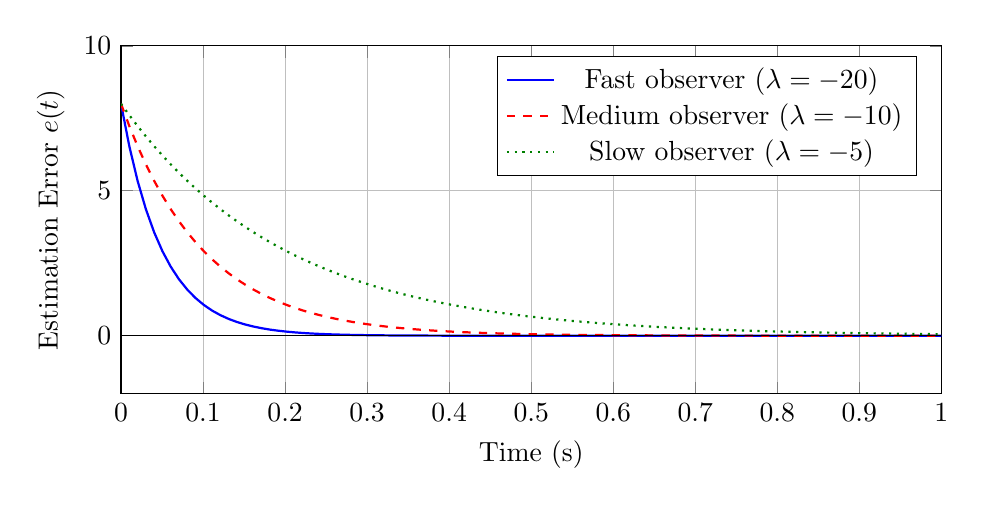
\begin{tikzpicture}
\begin{axis}[
    width=12cm,
    height=6cm,
    xlabel={Time (s)},
    ylabel={Estimation Error $e(t)$},
    legend pos=north east,
    grid=both,
    xmin=0, xmax=1,
    ymin=-2, ymax=10
]

% Fast observer (poles at -20)
\addplot[blue, thick, domain=0:1, samples=100]
    {8*exp(-20*x)};
\addlegendentry{Fast observer ($\lambda = -20$)}

% Medium observer (poles at -10)
\addplot[red, thick, dashed, domain=0:1, samples=100]
    {8*exp(-10*x)};
\addlegendentry{Medium observer ($\lambda = -10$)}

% Slow observer (poles at -5)
\addplot[green!50!black, thick, dotted, domain=0:1, samples=100]
    {8*exp(-5*x)};
\addlegendentry{Slow observer ($\lambda = -5$)}

% Zero line
\addplot[black, thin] coordinates {(0,0) (1,0)};

\end{axis}
\end{tikzpicture}
\caption{Estimation error convergence for observers with different pole locations. Faster poles (more negative) yield faster convergence but increased noise sensitivity.}
\label{fig:error_convergence}
\end{figure}

%% ============================================================================
\section{Worked Examples}
%% ============================================================================

\begin{examplebox}[Checking Observability of a Third-Order System]
\textbf{Problem:} Determine whether the following system is observable:
\begin{equation}
A = \begin{bmatrix} 0 & 1 & 0 \\ 0 & 0 & 1 \\ -6 & -11 & -6 \end{bmatrix}, \quad
C = \begin{bmatrix} 1 & 0 & 0 \end{bmatrix}
\end{equation}

\textbf{Solution:}

Step 1: Construct the observability matrix $\mathcal{O} = [C; CA; CA^2]^T$.

\begin{align}
C &= \begin{bmatrix} 1 & 0 & 0 \end{bmatrix}
\end{align}

\begin{align}
CA &= \begin{bmatrix} 1 & 0 & 0 \end{bmatrix} \begin{bmatrix} 0 & 1 & 0 \\ 0 & 0 & 1 \\ -6 & -11 & -6 \end{bmatrix} = \begin{bmatrix} 0 & 1 & 0 \end{bmatrix}
\end{align}

\begin{align}
CA^2 &= (CA)A = \begin{bmatrix} 0 & 1 & 0 \end{bmatrix} \begin{bmatrix} 0 & 1 & 0 \\ 0 & 0 & 1 \\ -6 & -11 & -6 \end{bmatrix} = \begin{bmatrix} 0 & 0 & 1 \end{bmatrix}
\end{align}

Therefore:
\begin{equation}
\mathcal{O} = \begin{bmatrix} 1 & 0 & 0 \\ 0 & 1 & 0 \\ 0 & 0 & 1 \end{bmatrix}
\end{equation}

Step 2: Check the rank.

The observability matrix is the $3 \times 3$ identity matrix, so $\text{rank}(\mathcal{O}) = 3 = n$.

\textbf{Conclusion:} The system is \textbf{observable}.

\textit{Remark:} This system is in \textbf{observer canonical form}. Systems in this form are always observable, just as systems in controller canonical form are always controllable.
\end{examplebox}

\hrulefill

\begin{examplebox}[Luenberger Observer Design for DC Motor]

\textbf{Problem:} Design a Luenberger observer for the DC motor system with desired observer poles at $s = -40$ and $s = -50$.

\begin{equation}
A = \begin{bmatrix} 0 & 1 \\ 0 & -10 \end{bmatrix}, \quad
B = \begin{bmatrix} 0 \\ 50 \end{bmatrix}, \quad
C = \begin{bmatrix} 1 & 0 \end{bmatrix}
\end{equation}

\textbf{Solution:}

Step 1: Verify observability.
\begin{equation}
\mathcal{O} = \begin{bmatrix} C \\ CA \end{bmatrix} = \begin{bmatrix} 1 & 0 \\ 0 & 1 \end{bmatrix}
\end{equation}
$\text{rank}(\mathcal{O}) = 2$, so the system is observable.

Step 2: Let $L = \begin{bmatrix} l_1 \\ l_2 \end{bmatrix}$. Compute $A - LC$:
\begin{equation}
A - LC = \begin{bmatrix} 0 & 1 \\ 0 & -10 \end{bmatrix} - \begin{bmatrix} l_1 \\ l_2 \end{bmatrix} \begin{bmatrix} 1 & 0 \end{bmatrix}
= \begin{bmatrix} -l_1 & 1 \\ -l_2 & -10 \end{bmatrix}
\end{equation}

Step 3: Find the characteristic polynomial of $A - LC$:
\begin{align}
\det(sI - A + LC) &= \det\begin{bmatrix} s + l_1 & -1 \\ l_2 & s + 10 \end{bmatrix} \\
&= (s + l_1)(s + 10) + l_2 \\
&= s^2 + (10 + l_1)s + (10l_1 + l_2)
\end{align}

Step 4: The desired characteristic polynomial with poles at $-40$ and $-50$ is:
\begin{equation}
(s + 40)(s + 50) = s^2 + 90s + 2000
\end{equation}

Step 5: Match coefficients:
\begin{align}
10 + l_1 &= 90 \implies l_1 = 80 \\
10l_1 + l_2 &= 2000 \implies l_2 = 2000 - 800 = 1200
\end{align}

\textbf{Result:}
\begin{equation}
\boxed{L = \begin{bmatrix} 80 \\ 1200 \end{bmatrix}}
\end{equation}
\end{examplebox}

\hrulefill

\subsection{Example 3: Duality Between Controllability and Observability}

\textbf{Problem:} Consider the system:
\begin{equation}
A = \begin{bmatrix} -2 & 1 \\ 0 & -3 \end{bmatrix}, \quad
B = \begin{bmatrix} 1 \\ 1 \end{bmatrix}, \quad
C = \begin{bmatrix} 1 & 0 \end{bmatrix}
\end{equation}

(a) Check controllability of $(A, B)$. (b) Check observability of $(A^T, B^T)$. (c) Verify the duality relationship.

\textbf{Solution:}

(a) Controllability of $(A, B)$:
\begin{equation}
\mathcal{C} = \begin{bmatrix} B & AB \end{bmatrix}
\end{equation}

\begin{equation}
AB = \begin{bmatrix} -2 & 1 \\ 0 & -3 \end{bmatrix} \begin{bmatrix} 1 \\ 1 \end{bmatrix} = \begin{bmatrix} -1 \\ -3 \end{bmatrix}
\end{equation}

\begin{equation}
\mathcal{C} = \begin{bmatrix} 1 & -1 \\ 1 & -3 \end{bmatrix}
\end{equation}

\begin{equation}
\det(\mathcal{C}) = (1)(-3) - (-1)(1) = -3 + 1 = -2 \neq 0
\end{equation}

So $(A, B)$ is \textbf{controllable}.

(b) Observability of $(A^T, B^T)$:

\begin{equation}
A^T = \begin{bmatrix} -2 & 0 \\ 1 & -3 \end{bmatrix}, \quad
B^T = \begin{bmatrix} 1 & 1 \end{bmatrix}
\end{equation}

The observability matrix for $(A^T, B^T)$ is:
\begin{equation}
\mathcal{O}_{A^T, B^T} = \begin{bmatrix} B^T \\ B^T A^T \end{bmatrix}
\end{equation}

\begin{equation}
B^T A^T = \begin{bmatrix} 1 & 1 \end{bmatrix} \begin{bmatrix} -2 & 0 \\ 1 & -3 \end{bmatrix} = \begin{bmatrix} -1 & -3 \end{bmatrix}
\end{equation}

\begin{equation}
\mathcal{O}_{A^T, B^T} = \begin{bmatrix} 1 & 1 \\ -1 & -3 \end{bmatrix}
\end{equation}

\begin{equation}
\det(\mathcal{O}_{A^T, B^T}) = (1)(-3) - (1)(-1) = -3 + 1 = -2 \neq 0
\end{equation}

So $(A^T, B^T)$ is \textbf{observable}.

(c) Verification of duality:

Note that $\mathcal{O}_{A^T, B^T} = \mathcal{C}_{A,B}^T$:
\begin{equation}
\mathcal{C}^T = \begin{bmatrix} 1 & -1 \\ 1 & -3 \end{bmatrix}^T = \begin{bmatrix} 1 & 1 \\ -1 & -3 \end{bmatrix} = \mathcal{O}_{A^T, B^T}
\end{equation}

Since they have the same rank (both full rank), the duality is verified: $(A, B)$ controllable $\Leftrightarrow$ $(A^T, B^T)$ observable.

\hrulefill

\subsection{Example 4: Observer-Based Controller Design}

\textbf{Problem:} For the system in Example 2, design a complete observer-based controller with controller poles at $s = -5 \pm 5j$ and observer poles at $s = -40$ and $s = -50$ (already computed in Example 2).

\textbf{Solution:}

Step 1: Design the state feedback gain $K$.

From Example 2, the system matrices are:
\begin{equation}
A = \begin{bmatrix} 0 & 1 \\ 0 & -10 \end{bmatrix}, \quad
B = \begin{bmatrix} 0 \\ 50 \end{bmatrix}
\end{equation}

Let $K = \begin{bmatrix} k_1 & k_2 \end{bmatrix}$. Then:
\begin{equation}
A - BK = \begin{bmatrix} 0 & 1 \\ -50k_1 & -10 - 50k_2 \end{bmatrix}
\end{equation}

Characteristic polynomial:
\begin{equation}
\det(sI - A + BK) = s^2 + (10 + 50k_2)s + 50k_1
\end{equation}

Desired characteristic polynomial with poles at $-5 \pm 5j$:
\begin{equation}
(s + 5 - 5j)(s + 5 + 5j) = s^2 + 10s + 50
\end{equation}

Matching coefficients:
\begin{align}
10 + 50k_2 &= 10 \implies k_2 = 0 \\
50k_1 &= 50 \implies k_1 = 1
\end{align}

So $K = \begin{bmatrix} 1 & 0 \end{bmatrix}$.

Step 2: From Example 2, $L = \begin{bmatrix} 80 \\ 1200 \end{bmatrix}$.

Step 3: The complete observer-based compensator is:
\begin{align}
\dot{\hat{x}} &= (A - BK - LC)\hat{x} + Ly \\
u &= -K\hat{x}
\end{align}

Computing $A - BK - LC$:
\begin{align}
A - BK &= \begin{bmatrix} 0 & 1 \\ -50 & -10 \end{bmatrix} \\
LC &= \begin{bmatrix} 80 \\ 1200 \end{bmatrix} \begin{bmatrix} 1 & 0 \end{bmatrix} = \begin{bmatrix} 80 & 0 \\ 1200 & 0 \end{bmatrix} \\
A - BK - LC &= \begin{bmatrix} -80 & 1 \\ -1250 & -10 \end{bmatrix}
\end{align}

\textbf{Complete Compensator:}
\begin{equation}
\boxed{
\begin{aligned}
\dot{\hat{x}} &= \begin{bmatrix} -80 & 1 \\ -1250 & -10 \end{bmatrix} \hat{x} + \begin{bmatrix} 80 \\ 1200 \end{bmatrix} y \\
u &= -\begin{bmatrix} 1 & 0 \end{bmatrix} \hat{x} = -\hat{x}_1
\end{aligned}
}
\end{equation}

Step 4: Verify closed-loop poles (separation principle).

The closed-loop eigenvalues consist of the controller poles at $-5 \pm 5j$ (eigenvalues of $A - BK$) and the observer poles at $-40$ and $-50$ (eigenvalues of $A - LC$). All four eigenvalues have negative real parts, confirming stability.

\hrulefill

\subsection{Example 5: Observer Convergence Rate Analysis}

\textbf{Problem:} For the observer designed in Example 2 with $L = [80; 1200]^T$, determine (a) the time for the estimation error to decay to 1\% of its initial value, and (b) the effect of doubling the observer gains on convergence time.

\textbf{Solution:}

(a) The estimation error dynamics are governed by:
\begin{equation}
A - LC = \begin{bmatrix} -80 & 1 \\ -1200 & -10 \end{bmatrix}
\end{equation}

The eigenvalues were designed to be $\lambda_1 = -40$ and $\lambda_2 = -50$.

For an initial error $e(0)$, the error decays as:
\begin{equation}
\|e(t)\| \approx \|e(0)\| e^{\lambda_{dom} t}
\end{equation}

where $\lambda_{dom} = -40$ is the dominant (slowest) eigenvalue.

For 1\% decay: $e^{-40t} = 0.01$
\begin{equation}
t = \frac{\ln(100)}{40} = \frac{4.605}{40} \approx 0.115 \text{ seconds}
\end{equation}

More conservatively, using the settling time formula ($t_s = 4/|\lambda_{dom}|$ for 2\%):
\begin{equation}
t_{1\%} \approx \frac{4.6}{40} = 0.115 \text{ seconds}
\end{equation}

(b) Doubling the observer gains changes the poles. Let $L' = 2L = [160; 2400]^T$.

New characteristic polynomial of $A - L'C$:
\begin{equation}
s^2 + (10 + 160)s + (10 \times 160 + 2400) = s^2 + 170s + 4000
\end{equation}

New poles: $s = \frac{-170 \pm \sqrt{170^2 - 4 \times 4000}}{2} = \frac{-170 \pm \sqrt{28900 - 16000}}{2} = \frac{-170 \pm 113.6}{2}$

\begin{equation}
\lambda_1' = -28.2, \quad \lambda_2' = -141.8
\end{equation}

The dominant pole is now at $-28.2$, which is actually slower than before! The new settling time:
\begin{equation}
t_{1\%}' \approx \frac{4.6}{28.2} = 0.163 \text{ seconds}
\end{equation}

\textbf{Key Insight:} Simply scaling the observer gains does not necessarily improve convergence. The pole locations depend on the specific structure of the gains, not just their magnitude. Proper pole placement requires careful computation, not ad-hoc gain adjustment.

\hrulefill

\subsection{Example 6: Unobservable System Analysis}

\textbf{Problem:} Consider the system:
\begin{equation}
A = \begin{bmatrix} -1 & 0 \\ 0 & -2 \end{bmatrix}, \quad
C = \begin{bmatrix} 1 & 1 \end{bmatrix}
\end{equation}

(a) Check observability. (b) If unobservable, identify the unobservable mode.

\textbf{Solution:}

(a) Construct the observability matrix:
\begin{align}
C &= \begin{bmatrix} 1 & 1 \end{bmatrix} \\
CA &= \begin{bmatrix} 1 & 1 \end{bmatrix} \begin{bmatrix} -1 & 0 \\ 0 & -2 \end{bmatrix} = \begin{bmatrix} -1 & -2 \end{bmatrix}
\end{align}

\begin{equation}
\mathcal{O} = \begin{bmatrix} 1 & 1 \\ -1 & -2 \end{bmatrix}
\end{equation}

\begin{equation}
\det(\mathcal{O}) = (1)(-2) - (1)(-1) = -2 + 1 = -1 \neq 0
\end{equation}

Since $\det(\mathcal{O}) \neq 0$, the rank is 2, and the system is \textbf{observable}.

Wait---let us reconsider. Consider instead:
\begin{equation}
A = \begin{bmatrix} -1 & 0 \\ 0 & -2 \end{bmatrix}, \quad
C = \begin{bmatrix} 1 & -1 \end{bmatrix}
\end{equation}

Then:
\begin{align}
CA &= \begin{bmatrix} 1 & -1 \end{bmatrix} \begin{bmatrix} -1 & 0 \\ 0 & -2 \end{bmatrix} = \begin{bmatrix} -1 & 2 \end{bmatrix}
\end{align}

\begin{equation}
\mathcal{O} = \begin{bmatrix} 1 & -1 \\ -1 & 2 \end{bmatrix}
\end{equation}

\begin{equation}
\det(\mathcal{O}) = (1)(2) - (-1)(-1) = 2 - 1 = 1 \neq 0
\end{equation}

Still observable. Let us try:
\begin{equation}
C = \begin{bmatrix} 1 & 2 \end{bmatrix}
\end{equation}

\begin{align}
CA &= \begin{bmatrix} 1 & 2 \end{bmatrix} \begin{bmatrix} -1 & 0 \\ 0 & -2 \end{bmatrix} = \begin{bmatrix} -1 & -4 \end{bmatrix}
\end{align}

\begin{equation}
\mathcal{O} = \begin{bmatrix} 1 & 2 \\ -1 & -4 \end{bmatrix}
\end{equation}

\begin{equation}
\det(\mathcal{O}) = (1)(-4) - (2)(-1) = -4 + 2 = -2 \neq 0
\end{equation}

Still observable. Let us use a truly unobservable example:

\textbf{Revised Problem:} Consider:
\begin{equation}
A = \begin{bmatrix} -1 & 1 \\ 0 & -1 \end{bmatrix}, \quad
C = \begin{bmatrix} 0 & 1 \end{bmatrix}
\end{equation}

\begin{align}
CA &= \begin{bmatrix} 0 & 1 \end{bmatrix} \begin{bmatrix} -1 & 1 \\ 0 & -1 \end{bmatrix} = \begin{bmatrix} 0 & -1 \end{bmatrix}
\end{align}

\begin{equation}
\mathcal{O} = \begin{bmatrix} 0 & 1 \\ 0 & -1 \end{bmatrix}
\end{equation}

\begin{equation}
\det(\mathcal{O}) = (0)(-1) - (1)(0) = 0
\end{equation}

Now $\text{rank}(\mathcal{O}) = 1 < 2$, so the system is \textbf{not observable}.

(b) To find the unobservable mode, we find the null space of $\mathcal{O}$:
\begin{equation}
\mathcal{O} v = 0 \implies \begin{bmatrix} 0 & 1 \\ 0 & -1 \end{bmatrix} \begin{bmatrix} v_1 \\ v_2 \end{bmatrix} = 0
\end{equation}

This gives $v_2 = 0$, so any $v = \begin{bmatrix} \alpha \\ 0 \end{bmatrix}$ with $\alpha \neq 0$ is in the null space.

The unobservable state is the first state $x_1$. Any initial condition of the form $x_0 = [x_{10}, 0]^T$ will produce $y(t) = 0$ for all $t$, making $x_{10}$ indeterminate from output measurements alone.

\textbf{Physical interpretation:} The mode associated with $x_1$ is ``hidden'' from the output. We can only observe $x_2$ and its evolution. The coupling from $x_1$ to $x_2$ (the ``1'' in position $(1,2)$ of $A$) is one-directional and does not help because we cannot see $x_1$ directly, and $x_1$ does not affect $\dot{x}_2$.

%% ============================================================================
\section{Summary}
%% ============================================================================

This chapter introduced the fundamental concept of observability and the practical technique of state estimation using Luenberger observers.

\subsection{Key Concepts}

\textbf{Observability} answers the fundamental question: can we determine the system's internal state from measurements of its output? The \textbf{observability matrix} $\mathcal{O} = [C; CA; \ldots; CA^{n-1}]^T$ provides a test for this property---a system is observable if and only if $\text{rank}(\mathcal{O}) = n$.

A key theoretical insight is the \textbf{duality} between observability and controllability: $(A, C)$ is observable if and only if $(A^T, C^T)$ is controllable. This duality connects the two fundamental structural properties of linear systems.

The \textbf{Luenberger observer} estimates unmeasured states using the equation:
\begin{equation}
\dot{\hat{x}} = A\hat{x} + Bu + L(y - C\hat{x})
\end{equation}
The estimation error dynamics are governed by $(A - LC)$, and the observer gain $L$ can be designed to place the eigenvalues at any desired locations if the system is observable.

The \textbf{separation principle} allows independent design of the controller gain $K$ and observer gain $L$; the combined closed-loop system's eigenvalues are simply the union of the controller and observer eigenvalues. In practice, observer poles should be placed faster than controller poles (typically 2--10 times) but not so fast as to amplify measurement noise excessively.

\subsection{Design Procedure}

The observer design procedure follows a systematic approach. First, verify observability using the rank condition on the observability matrix. Then select desired observer pole locations, ensuring they are faster than the controller poles. Next, compute the observer gain $L$ using pole placement methods such as Ackermann's formula, the \texttt{place} command, or manual coefficient matching. Implement the observer in software or hardware, and finally use the estimated states for state-feedback control via $u = -K\hat{x}$.

\subsection{Looking Ahead}

The Luenberger observer assumes perfect knowledge of the system model and deterministic operation. In Chapter 17, we will study the Linear Quadratic Regulator (LQR), which provides optimal state feedback. In Chapter 18, we will introduce the Kalman filter, which extends the observer concept to handle model uncertainty and measurement noise optimally.

%% ============================================================================
\newpage
\section{Exercises}
%% ============================================================================

\begin{exercise}
Consider the system with:
\begin{equation}
A = \begin{bmatrix} 0 & 1 & 0 \\ 0 & 0 & 1 \\ -1 & -3 & -3 \end{bmatrix}, \quad
C = \begin{bmatrix} 1 & 0 & 0 \end{bmatrix}
\end{equation}
\begin{enumerate}
    \item[(a)] Determine whether the system is observable.
    \item[(b)] If observable, design an observer with all poles at $s = -10$.
\end{enumerate}
\end{exercise}

\begin{exercise}
For the double integrator $\ddot{y} = u$ with output $y$ (position only):
\begin{enumerate}
    \item[(a)] Write the state-space model.
    \item[(b)] Check observability.
    \item[(c)] Design an observer with poles at $s = -5 \pm 5j$.
    \item[(d)] Simulate the observer response to an initial position error of 1 meter.
\end{enumerate}
\end{exercise}

\begin{exercise}
Prove that a system in observer canonical form is always observable.
\end{exercise}

\begin{exercise}
A system has open-loop poles at $s = -1$ and $s = -2$, and a controller has been designed with closed-loop poles at $s = -5 \pm 3j$. What observer pole locations would you recommend, and why?
\end{exercise}

\begin{exercise}
For the observer-based controller in Example 4:
\begin{enumerate}
    \item[(a)] Write the compensator as a transfer function from $y$ to $u$.
    \item[(b)] Sketch the Bode plot of the compensator.
    \item[(c)] Analyze the stability margins of the closed-loop system.
\end{enumerate}
\end{exercise}

\begin{exercise}
Consider a system with:
\begin{equation}
A = \begin{bmatrix} -1 & 0 & 0 \\ 0 & -2 & 0 \\ 1 & 1 & -3 \end{bmatrix}, \quad
C = \begin{bmatrix} 0 & 0 & 1 \end{bmatrix}
\end{equation}
\begin{enumerate}
    \item[(a)] Determine observability.
    \item[(b)] Identify any unobservable modes.
    \item[(c)] What physical interpretation might explain why these modes are unobservable?
\end{enumerate}
\end{exercise}

\begin{exercise}
(Computer Exercise) Implement the motor velocity observer from the practical experiment in MATLAB/Simulink. Add measurement noise to the position signal and compare the noise sensitivity of:
\begin{enumerate}
    \item[(a)] Numerical differentiation
    \item[(b)] Numerical differentiation with low-pass filter
    \item[(c)] Luenberger observer with different pole locations
\end{enumerate}
Plot the trade-off between convergence speed and noise amplification.
\end{exercise}

\begin{exercise}
Derive the transfer function from measurement $y$ to state estimate $\hat{x}$ for a Luenberger observer. Show that as the observer poles approach infinity (infinitely fast observer), this transfer function approaches the ``pseudo-inverse'' relationship $\hat{x} \approx \mathcal{O}^{-1}[y; \dot{y}; \ldots]$.
\end{exercise}

\begin{exercise}
Consider a system where the output is a linear combination of states:
\begin{equation}
A = \begin{bmatrix} -2 & 1 \\ 0 & -3 \end{bmatrix}, \quad
C = \begin{bmatrix} 1 & 1 \end{bmatrix}
\end{equation}
\begin{enumerate}
    \item[(a)] Verify the system is observable.
    \item[(b)] Design an observer with poles at $s = -10$ and $s = -12$.
    \item[(c)] Compare the transient response of this observer with one having poles at $s = -5$ and $s = -6$.
\end{enumerate}
\end{exercise}

\begin{exercise}
\textbf{(Reduced-Order Observer)} For a second-order system where position is measured but velocity is not, design a first-order reduced-order observer that estimates only the unmeasured velocity state. Compare its performance with a full-order observer.
\end{exercise}

%% ============================================================================
%% End of Chapter 16
%% ============================================================================
